\section{Appendix}
\label{sec:appendix}

 \begin{figure}[h!]
  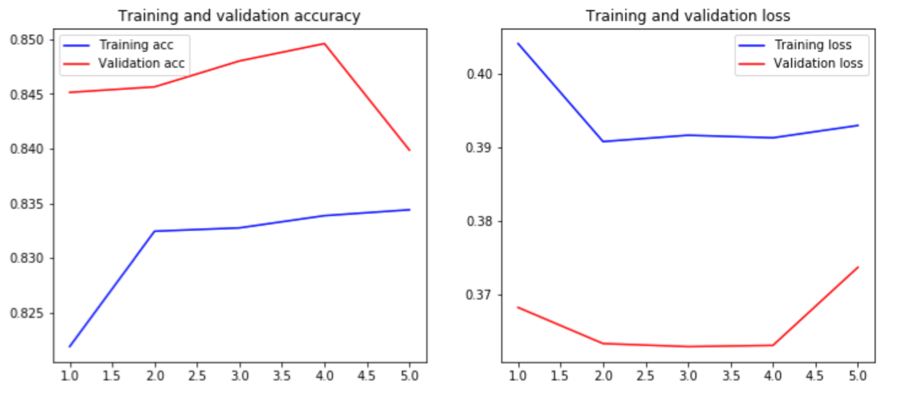
\includegraphics{multilayers.png}
  \caption{multiple hidden layered feed-forward neural network approach with pre-trained GloVE embedding where x-axis is the epochs and y-axis is: the accuracy on the left and the loss on the right}
  \label{fig:nnpre}
\end{figure} 

\begin{figure}[h!]
  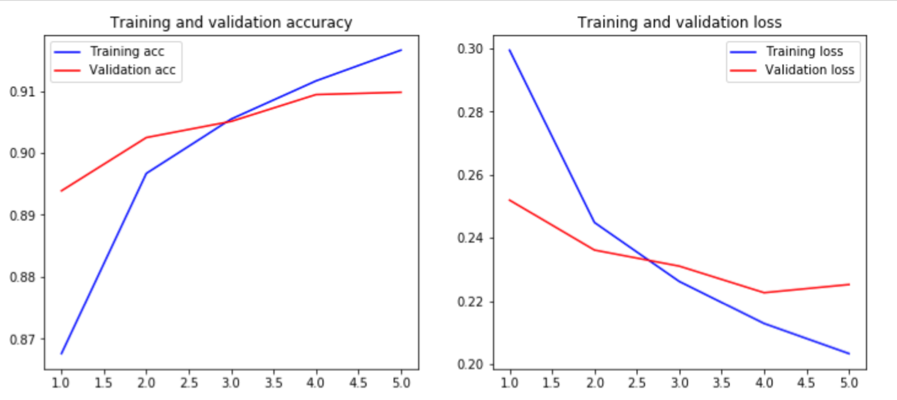
\includegraphics[width=\linewidth]{LSTM400.png}
  \caption{LSTM layer with 400 neurons where x-axis is the epochs and y-axis is: the accuracy in left and the loss on the right.}
  \label{fig:lstm400}
\end{figure}  

\begin{figure}[h!]
  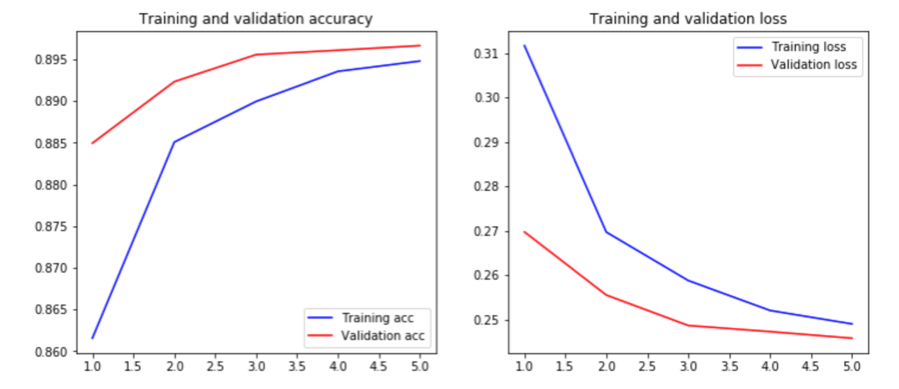
\includegraphics[width=\linewidth]{train90.png}
  \caption{LSTM model with 90\% for training data where x-axis is the epochs and y-axis is: the accuracy on the left and the loss on the right.}
  \label{fig:lstm90}
\end{figure} 

\begin{figure}[h!]
  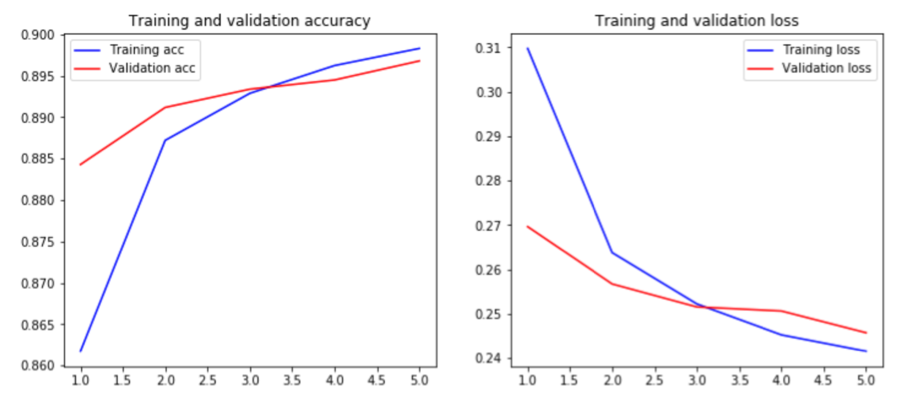
\includegraphics[width=\linewidth]{vocabChange.png}
  \caption{LSTM with embedding dictionary that doesn't have vocabularies from the validation data where x-axis is the epochs and y-axis is: the accuracy on the left and the loss on the right .}
  \label{fig:lstmvoc}
\end{figure} . 
